\subsection{Network of Agents}\label{subsec:network}
Our network is made of Agents eventually connected by weighted and undirected links.
At the first time, the network is composed by the sum of a fixed number of sources and users. \\
Users are linked with a fixed probability computed from the desired average degree and inserted by external input.
 In this way we obtain a random network of users, with exponential trend for the degree distribution in the termodynamic limit.
\\ Links are the only possibility to establish a relation between the agents; a random value of weight of the link represents a previous bias in 
friendship.\footnote{This particular choice for our links underlines bilaterality and intensity of communication between agents.
Taking as example an exchange of information between two people or between a person and a newspaper, weight represents feeling, previous chemistry;}
The result of such a mechanism of graph generation doesn't actually return a real network, because social real networks possess the property of 
scale-free;\footnote{The scale-free property is mainly described by power law degree distribution, with a cut-off for high degrees (i.e. hubs). } instead, random graphs have a majority of node-degrees peaked around the average-degree. 
Also, the variance is very large in scale-free network and guarantees the existence of hubs in the network.\cite{newman1963introduction}
Despite the abovementioned theory, we start with a random network hoping to observe a natural evolution in this direction.

Sources are a news reservoir: users can pick one or more news from them and eventually spread.
Sources' degree is higher than users' one because we assume that newspapers have more links than a common user.
Sources contain a fixed number of news and eventually regenerate them run-time. \\
Each single news contains: a unique string which identifies it, a vector of topics, the initial source's ID, creation date, its own relevance (a sort of "impact factor").

Users own a vector, the "state of mind", representing their own personality: sources, like users, have a "personality" too (i.e. another vector), which reflects news' content.
Users can remember a limited number of news, according to the affinity between incoming news and their state of mind.
Furthermore, affinity also regulates diffusion by users.
State of mind is not fixed but it is affected by news spreading; links' weights can be modified by users' state of mind.
Time is externally imposed and, according to it, users can be active or inactive: only when active, they can interact with external world.

\begin{figure}[htpb]
  \centering
  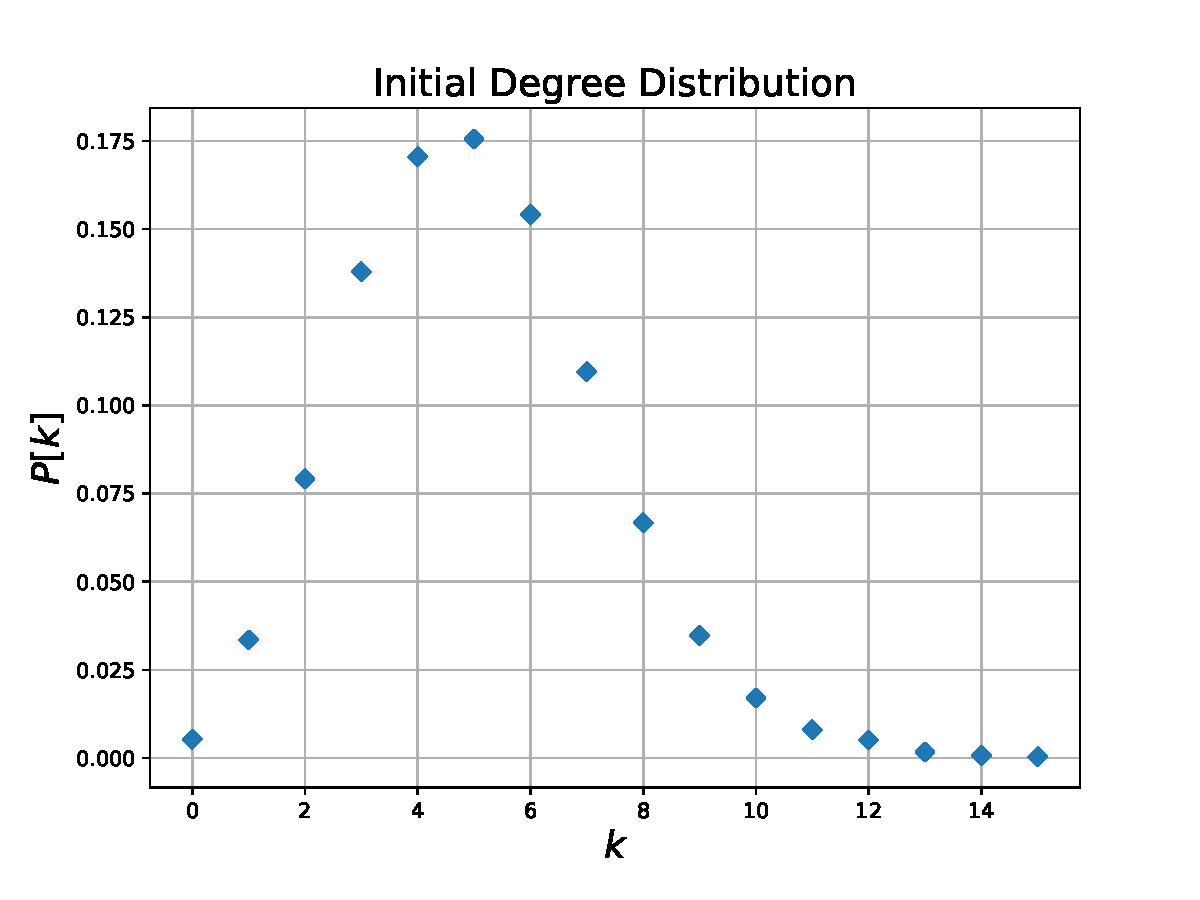
\includegraphics[width=\columnwidth]{img/pdf/gauss.pdf}
  \caption{Degree Distribution, seed 17, 3 sources, 10000 users, 5 initial average degree, 1 time step}
  \label{fig:gauss}
\end{figure}
